\section{Instruction Size}
We ended up with a 24-bit instruction set for both \ac{SIMD} nodes and the
control core. As we had a 16-bit program counter, the maximal
instruction count would be 64k and the memory chip size is chosen on that
basis. While it may sound little, it is still more than enough. We usually
write programs for a single frame, without any concern for
the one coming after it. The program is simply restarted for every new frame,
reducing the amount of code needed and the complexity of the programs.

\section {Memory Architecture}
\begin{figure}[h]
  \centering
  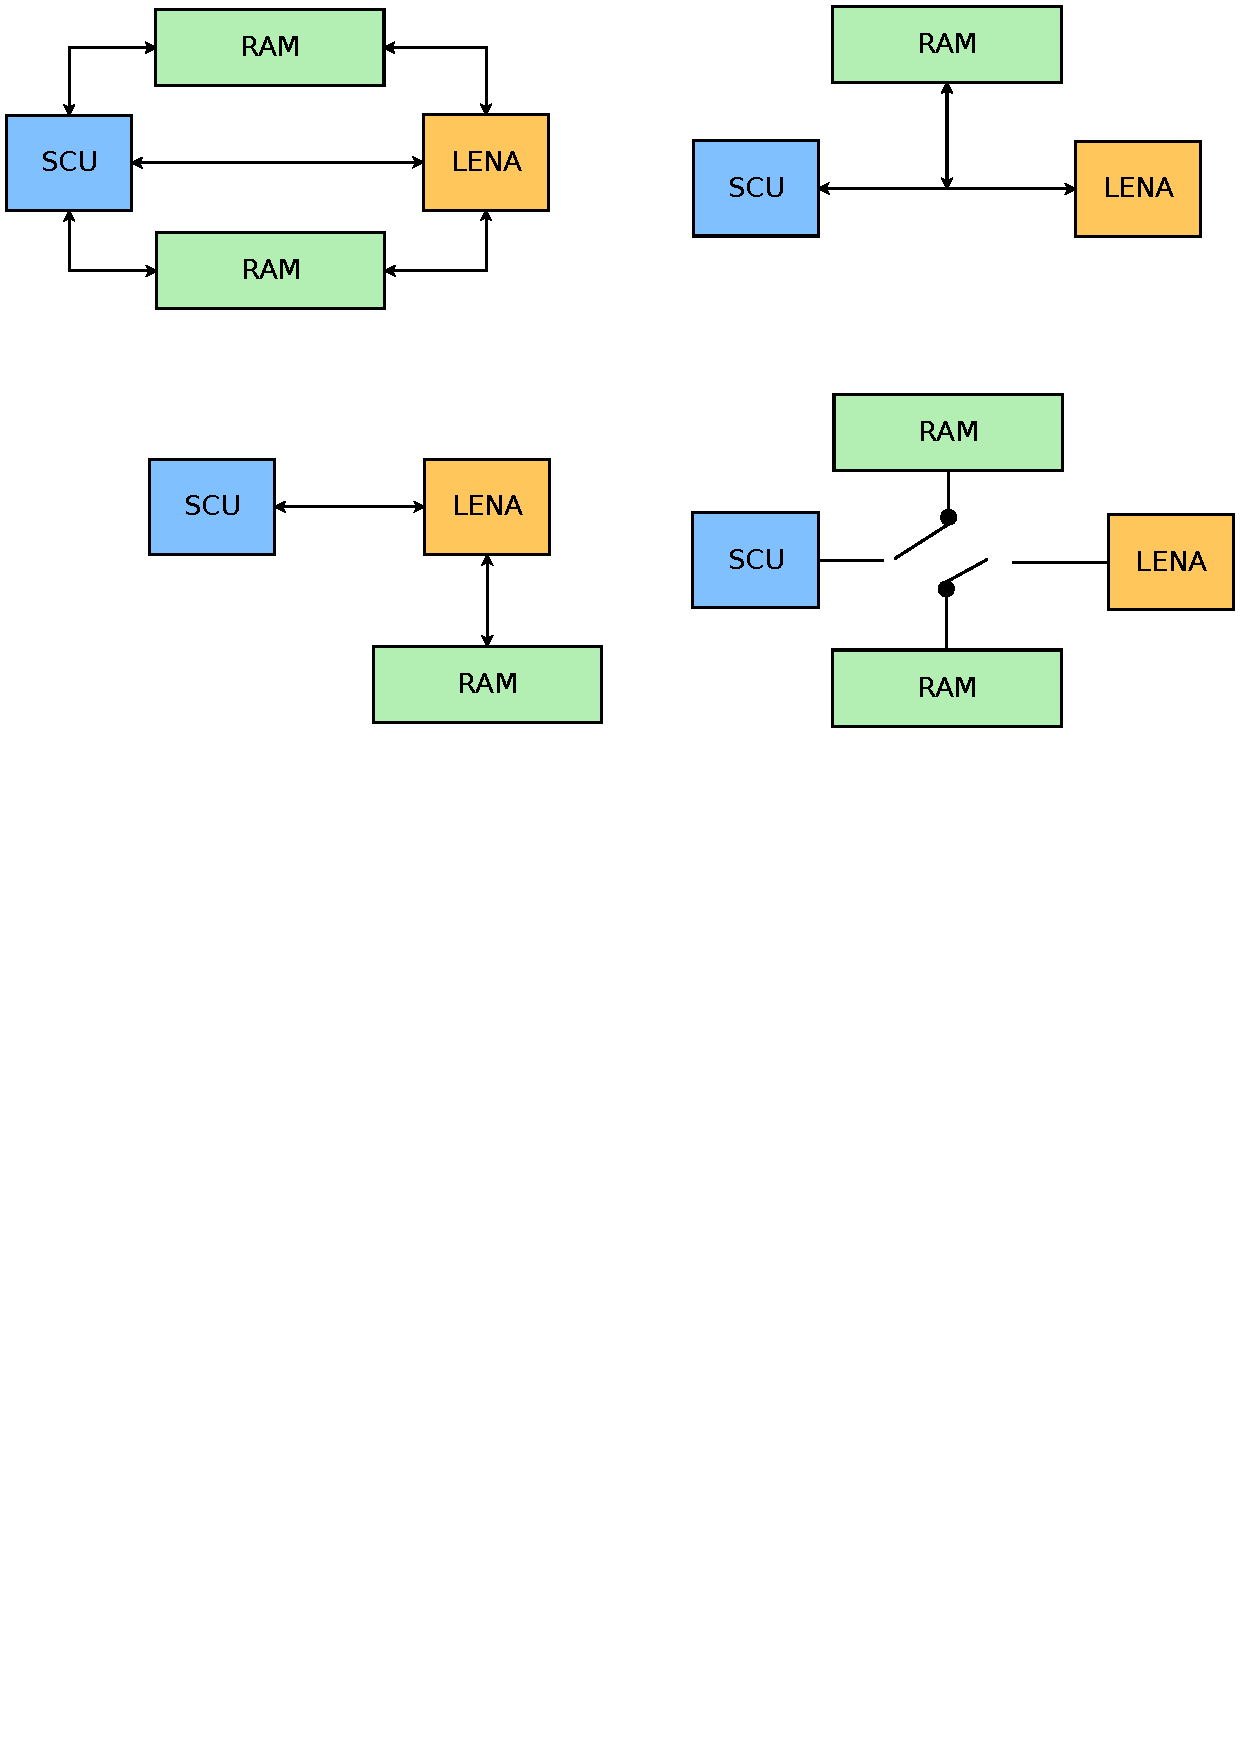
\includegraphics[width=0.8\textwidth]{fig/disc/memarch.pdf}
  \caption[Data Memory Architecturres]{Considered data memory architectures}
  \label{fig:memarch}
\end{figure}
 

In the early phases of the project, multiple solutions as to how the data memory
should work were suggested. 

The top left example of Figure \ref{fig:disc-memarch} shows a shared memory architecture with separate data and
instruction memories. The top right example shows one single memory connected to
both the SCU and LENA by a common bus. In the bottom left example, the memory is
only connected to the LENA, and the SCU communicates with it through LENA. 
The bottom right example shows a switched memory architecture. There are two memories
that can both be connected to the SCU and to the LENA, but not at the same time.

We decided to let the \ac{SCU} send all the data to
the \ac{LENA}, and then let it store them to its own local memory, like in the bottom left example. The reason we
chose this over shared memory was all the potential issues we might get with the
shared memory solution. A shared memory would be prone to errors from
synchronization problems such as knowing when, and to which addresses, a
read/write operation should happen.

To allow overlap between loading instructions and data in the LENA architecture,
we chose the Harvard Architecture and used a separate memory for
instructions. The program memory is separated into two chips. The reason for
this is mainly that we found no good 24 bit word memory (24 bit to match instruction
size). One solution would be to just buy a 32 bit memory. However, a single 32 bit
memory was more expensive than two 16 bit memories. As both gave us the needed
memory, we chose the cheaper alternative.

In addition, we figured a shared \ac{VGA} and data memory would obstruct the
flow of data from the \ac{SCU}. Since data for the \ac{VGA} would be both read
and written frequently, the \ac{VGA} needed its own memory, rather than sharing
memory with the rest of the LENA architecture. We
therefore invested in an extra memory chip. For the VGA we chose an 8-bit word
memory that was big enough to hold at least a full frame, at 8 bits per
pixel (since each pixel is an 8-bit greyscale pixel).

Finally, to reduce the possibility of having too slow data access from the SCU,
an extra memory was added to work as a buffer
for the SCU as well. This design choice was made {\em after} ordering, which
meant that we had to choose from the chips we had already ordered to fit this
purpose. Since this was intended to carry data to all other parts of the system,
and as the rest of the system is working with data in 8 bit words, we ended up
using one of the extra chips ordered as \ac{VGA} memory for this purpose.

A result of this is that we now had four separate memories to allow overlap of
memory accesses. Since the requirements for the data/instruction memories
differed in both size and word-width, we wound up with not only separate, but
also different chips for this purpose.

\section{Redundancies}
We had multiple redundancies to avoid potential errors which would have rendered
our whole system unusable. This was recommended by Jahre, and previous groups
had done so as well. In order to send data into the system, our two main options
would be to use the \ac{SD} card or the mini \ac{USB} plug. We had serial and
\ac{JTAG} for debugging purposes. For the graphical output we had the two
\ac{VGA} options. Luckily, both \ac{SD} card and and our own \ac{VGA} worked,
and we therefore never needed to use any of our redundant solutions.
